%-----------------------------------------------------------------------------
%
%               Template for sigplanconf LaTeX Class
%
% Name:         sigplanconf-template.tex
%
% Purpose:      A template for sigplanconf.cls, which is a LaTeX 2e class
%               file for SIGPLAN conference proceedings.
%
% Guide:        Refer to "Author's Guide to the ACM SIGPLAN Class,"
%               sigplanconf-guide.pdf
%
% Author:       Paul C. Anagnostopoulos
%               Windfall Software
%               978 371-2316
%               paul@windfall.com
%
% Created:      15 February 2005
%
%-----------------------------------------------------------------------------


\documentclass[preprint]{sigplanconf}

% The following \documentclass options may be useful:
%
% 10pt          To set in 10-point type instead of 9-point.
% 11pt          To set in 11-point type instead of 9-point.
% authoryear    To obtain author/year citation style instead of numeric.

\usepackage{amsmath}
\usepackage{graphicx}

\begin{document}

\conferenceinfo{WXYZ '05}{date, City.} 
\copyrightyear{2005} 
\copyrightdata{[to be supplied]} 

\titlebanner{banner above paper title}        % These are ignored unless
\preprintfooter{short description of paper}   % 'preprint' option specified.

\title{iMonitor: An Implicit-Signal Monitor}
\subtitle{}

\authorinfo{Name1}
           {Affiliation1}
           {Email1}
\authorinfo{Name2\and Name3}
           {Affiliation2/3}
           {Email2/3}

\maketitle

\begin{abstract}
This is the text of the abstract.
\end{abstract}

\category{CR-number}{subcategory}{third-level}

\terms
term1, term2

\keywords
keyword1, keyword2

\section{Introduction}

The text of the paper begins here.

\section{Background}
\section{Syntax and Framework of iMonitor}

\begin{figure}[h!]
  \centering
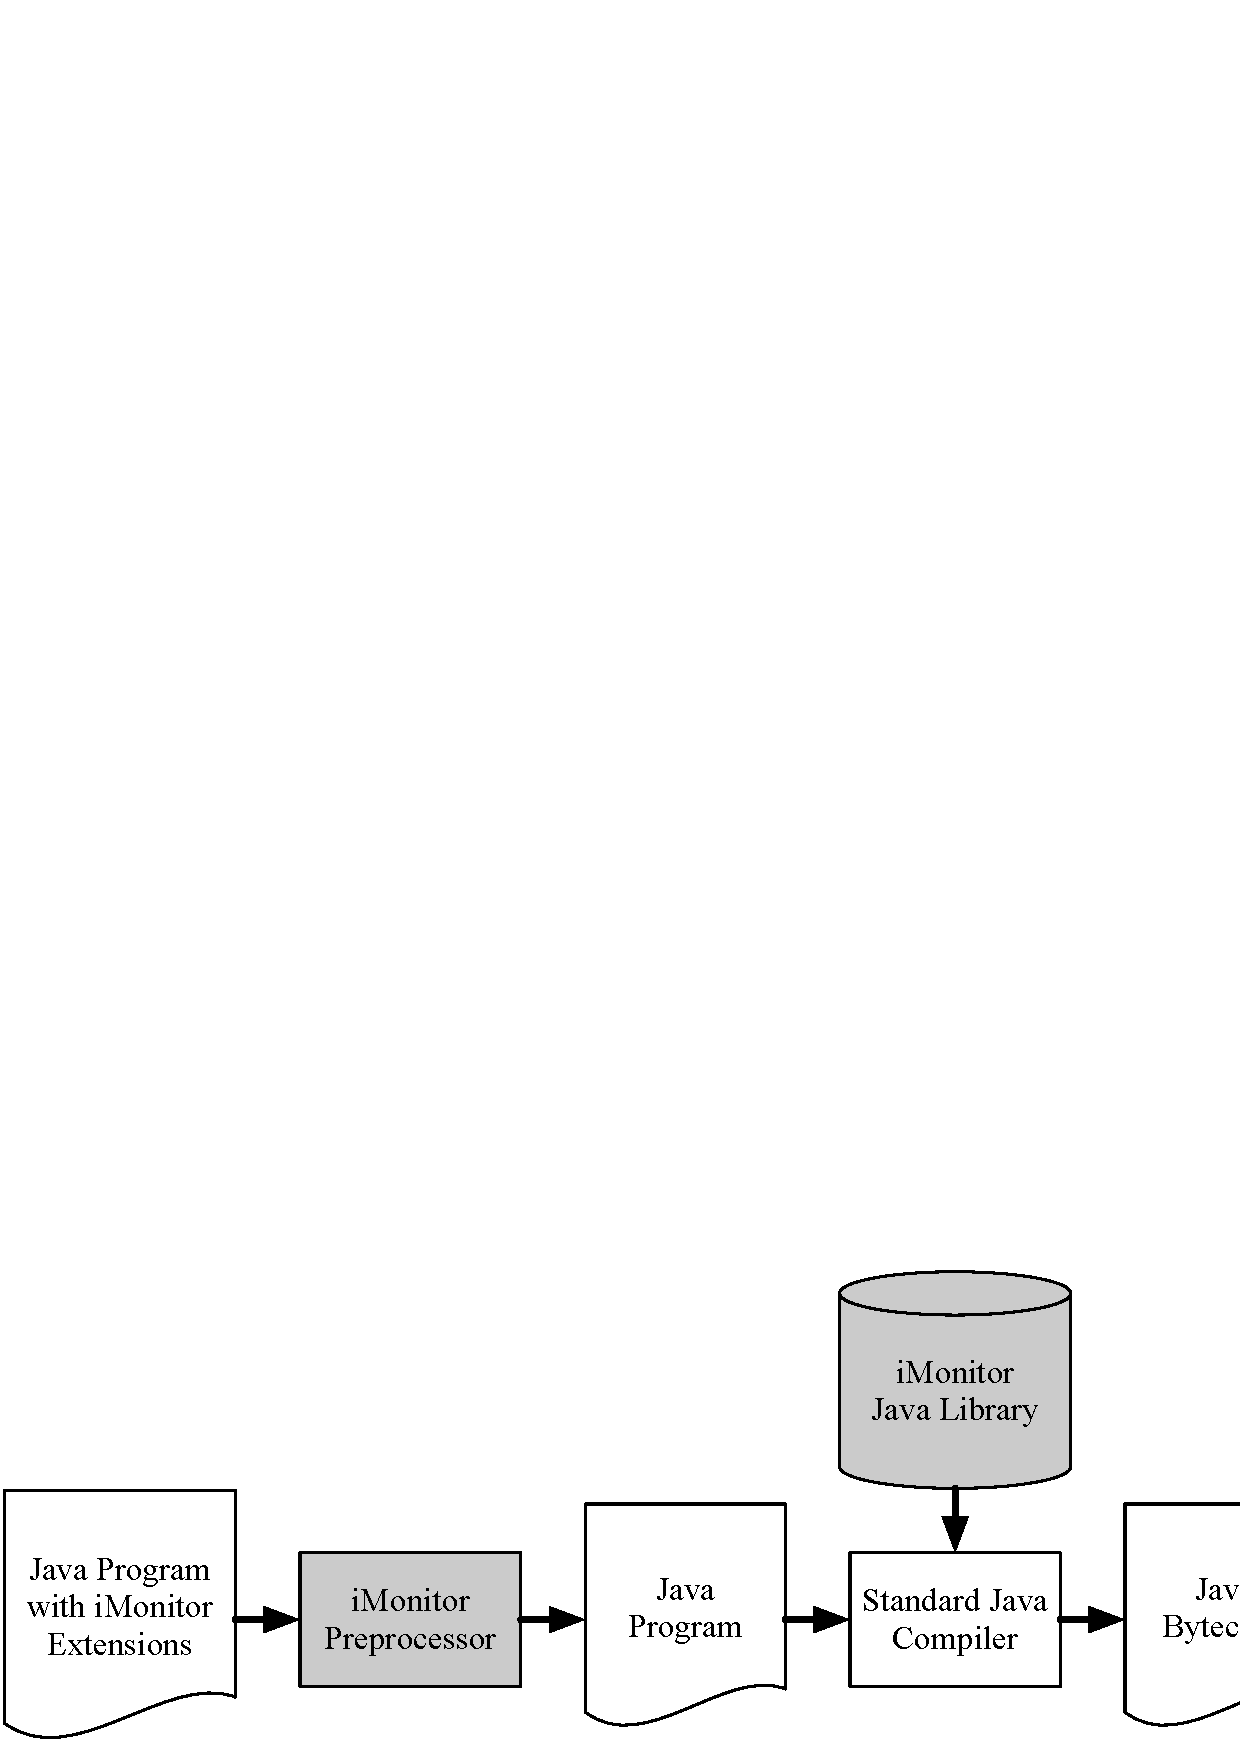
\includegraphics[width=70mm]{fig/flow.png}
\caption{The framework of iMonitor}
\end{figure}

\section{Details of Implicit-Signal Monitors}
\subsection{Naive}
\subsection{N-Condition}
\subsection{HashMap-Condition}
\subsection{Dependent-Condition} 
\section{Experimental Results}
\subsection{Bounded-Buffer Problem}
\subsection{Reader/Writer Problem}
\subsection{Dining Philosophers  Problem}
\subsection{Sleeping Barber Problem}
\subsection{Access Patterns}

\section{Conclusions}

\appendix
\section{Appendix Title}

This is the text of the appendix, if you need one.

\acks

Acknowledgments, if needed.

% We recommend abbrvnat bibliography style.

\bibliographystyle{abbrvnat}

% The bibliography should be embedded for final submission.

\begin{thebibliography}{}
\softraggedright

\bibitem[Buhr et~al.(2005)Buhr, P.A.]{bh05}
Buhr, P. A. and Harji, A. S. Implicit-Signal Monitors. ACM Transactions on Programming Languages and Systems, 27(6), 1270�1343. ACM. doi:10.1145/1108970.1108975

\end{thebibliography}

\end{document}
